% This is the root file of your thesis: thesis.tex
% A line starting with % is a comment. In some cases, I have included a command preceded by a %. You may activate the command by removing the %.

%%===================================
\documentclass[12pt, twoside, openright]{report}
\usepackage{ramsstyle}
\usepackage{float}
\usepackage{hyperref}
\usepackage{longtable}
\usepackage{subfigure}
\usepackage{tabularx}
\newcolumntype{C}[1]{>{\centering\arraybackslash}p{#1}}
\usepackage{pdfpages}
\usepackage{wrapfig}
\usepackage{tocbibind}
\usepackage[bottom]{footmisc}
%%===================================
%Write the various parts of your thesis as separate files and include them into the main file by the command \include{name of included file}. When you compile the LaTeX file, you may choose which subfiles to include by the command
%%===================================
\begin{document}
%\setcounter{page}{0}
%This is the Titlepage
%%=========================================
\thispagestyle{empty}

\includegraphics[scale=0.8]{fig/NTNU}
\mbox{}\\[2pc]
\begin{center}
\Huge{Drop and Recovery of Sensor Nodes Using UAVs}\\[3pc]

\Large{Vegard Voldsund}\\[1pc]
\large{June 2014}\\[4pc]

MASTER THESIS\\
Department of Engineering Cybernetics\\
Centre for Autonomous Marine Operations and Systems\\
Norwegian University of Science and Technology
\end{center}
%\begin{figure}[H]
%\center
%\includegraphics[width=10 cm]{fig/finished/finished.jpg}
%\end{figure}
\vfill

\noindent Supervisor 1: Professor Tor Arne Johansen 

\noindent Supervisor 2: PhD Candidate Kristian Klausen

 % This is the titlepage
\pagenumbering{roman}
\setcounter{page}{0}
%\chapter*{Problem Description}
%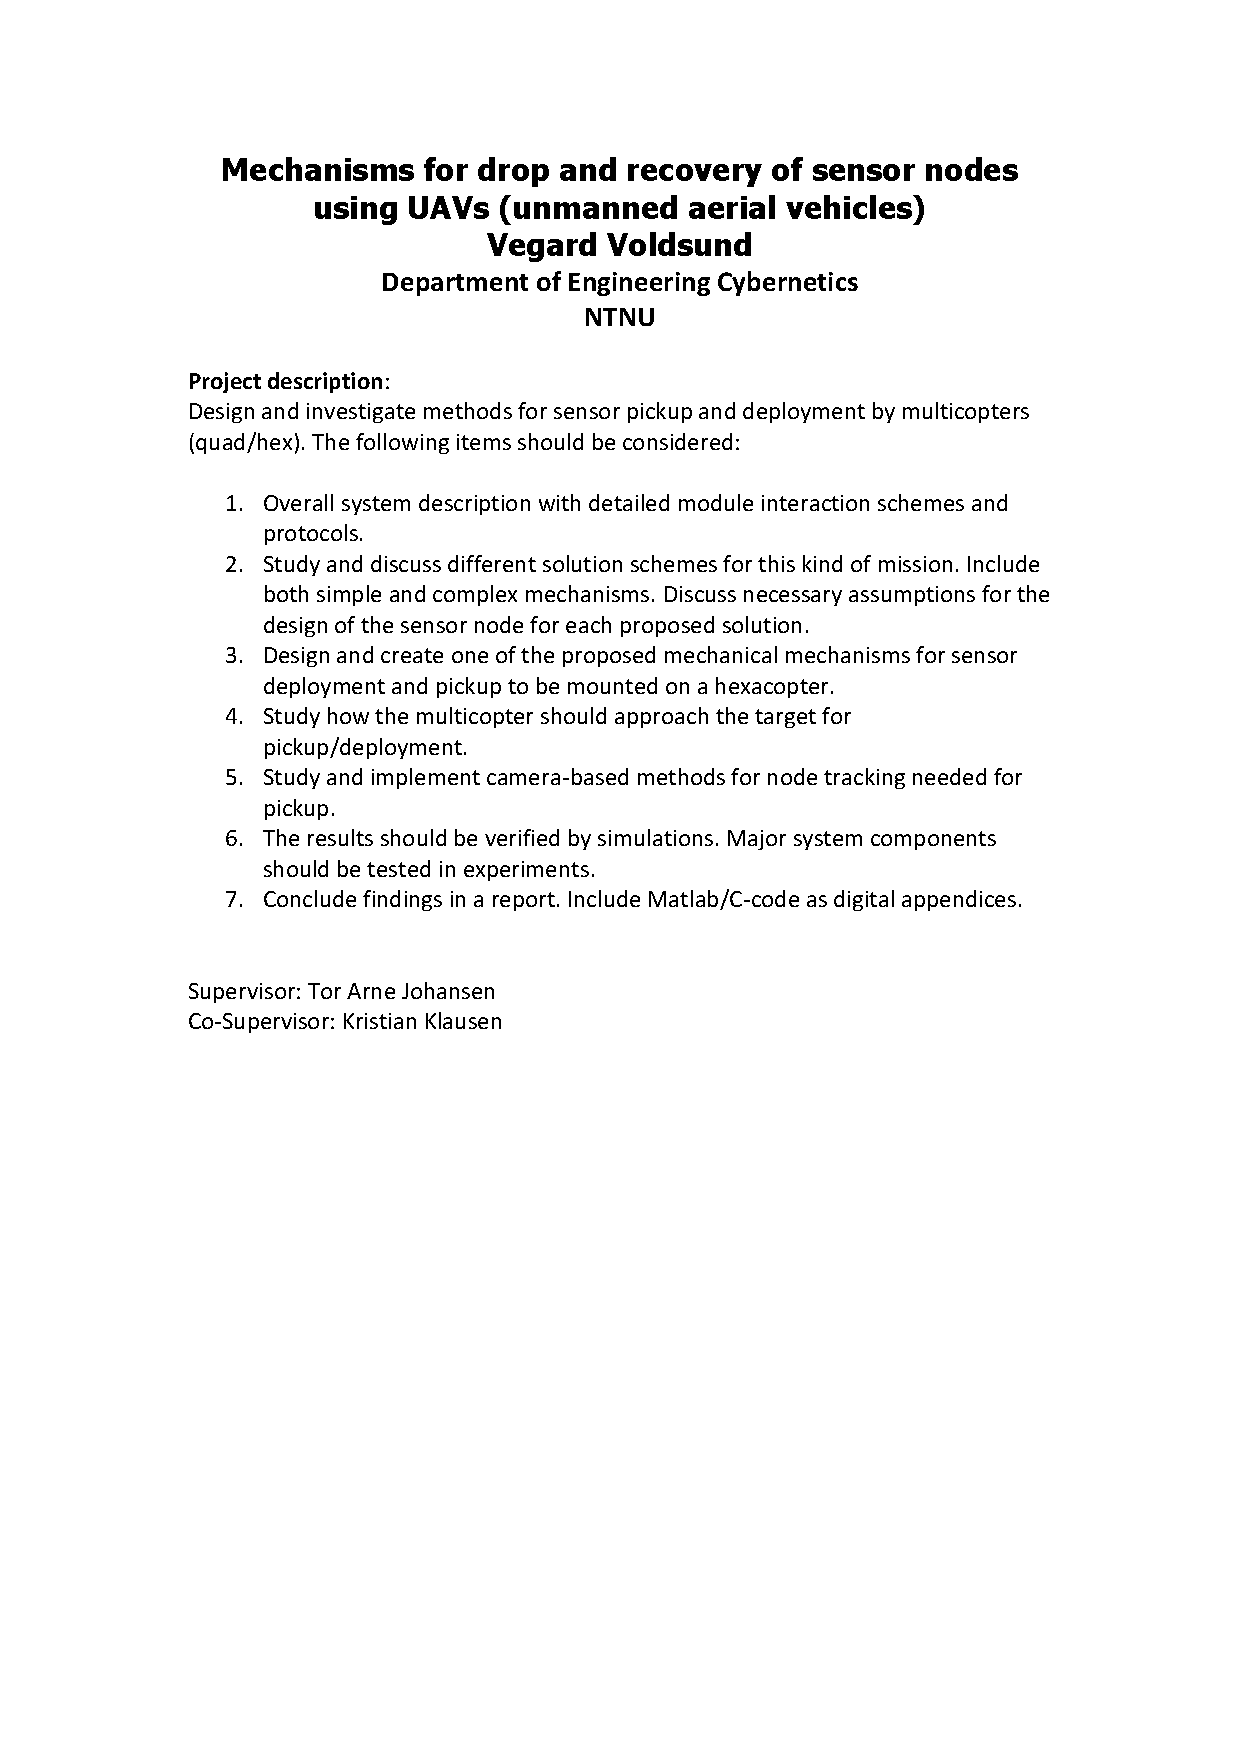
\includegraphics[scale=0.6]{oppgave.pdf}
\addcontentsline{toc}{chapter}{Problem Description}
\vspace*{\fill}
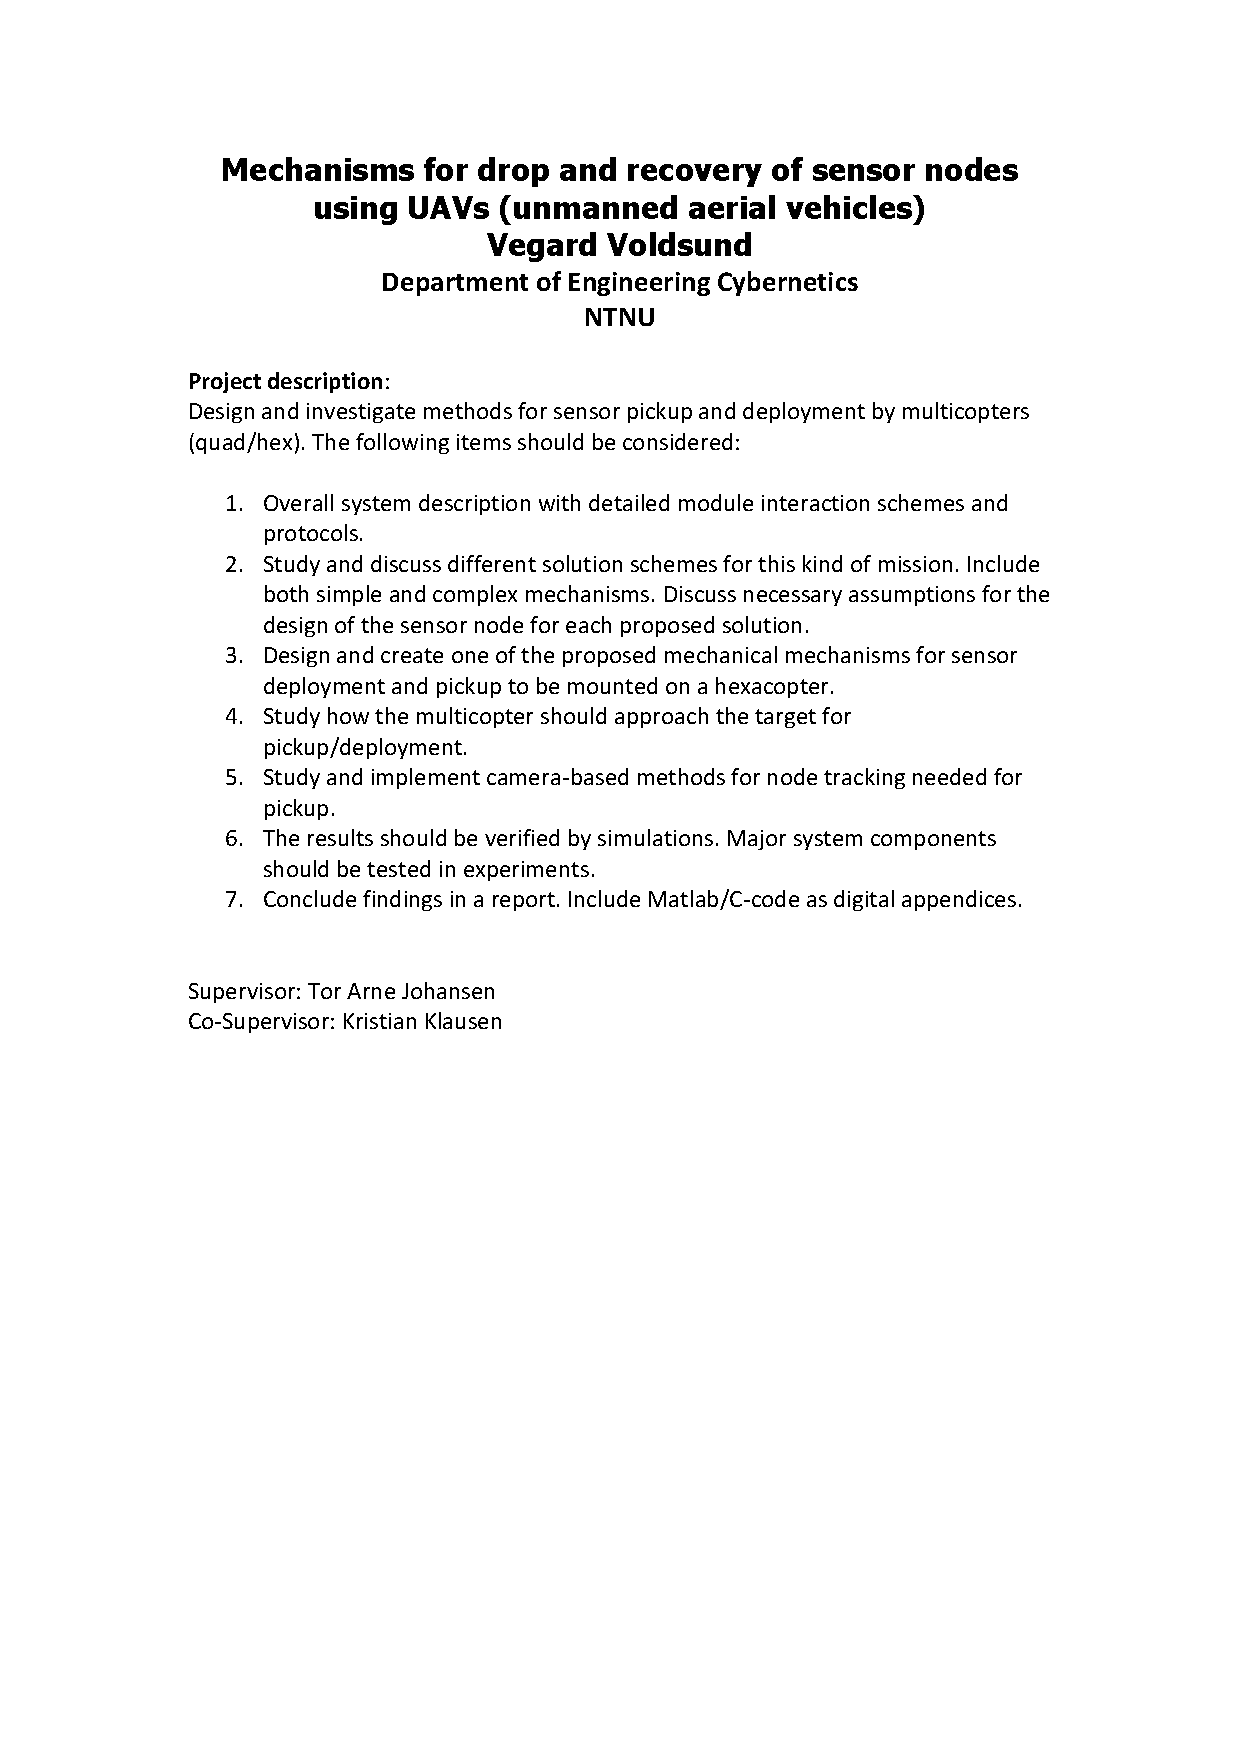
\includepdf[offset = 0cm -5cm, scale = 1, pages=1, pagecommand=\chapter*{Problem Description}]{oppgave.pdf}



\addcontentsline{toc}{chapter}{Abstract}
\chapter*{Abstract}

%This is the Summary
%%=========================================
\addcontentsline{toc}{chapter}{Sammendrag}
\chapter*{Sammendrag}
\textit{(Norwegian translation of the abstract)}\\
\newline

%This is the Preface
%%=========================================
\addcontentsline{toc}{chapter}{Preface}
\chapter*{Preface}
This project is written as a part of my MSc degree at the Department of Engineering Cybernetics at NTNU  and is part of research conducted by the Center of Autonomous Marine Operations and Systems (AMOS). The work in this project will be continued into my master thesis.\\
\newline
The execution of this project would not have been possible without the financial backing from AMOS and the usage of equipment at the electronics and mechanical workshops at the Department of Engineering Cybernetics, NTNU. I will like to thank the guys at these workshops for valuable help and guidance.\\
\newline
I would also like to thank my supervisors Professor Tor Arne Johansen and PhD Candidate Kristian Klausen for guidance and encouragement along the way.\\
\newline
\begin{flushright}
\textit{Vegard Voldsund}
\end{flushright}
%This is Appendix A - Acronyms
%%=========================================
\addcontentsline{toc}{chapter}{Acronyms}
\chapter*{Acronyms}
\begin{tabular}{l l}
\textbf{AMOS} & Centre for Autonomous Marine Operations and Systems\\
%\textbf{APM 2.6} & Ardupilot Mega 2.6\\
%\textbf{BGR} & Blue-Green-Red\\
%\textbf{CEP} & Circular Error Probability\\
%\textbf{CPU} & Central Processing Unit\\
%\textbf{DH Convention} & Denavit-Hartenberg Convention\\
%\textbf{ECEF} & Earth-centered Earth-fixed\\
%\textbf{GPS} & Global Positioning System\\
%\textbf{HSV} & Hue-Saturation-Value\\
%\textbf{IC} & Integrated Circuit\\
%\textbf{IMU} & Inertial Measurement Unit\\
%\textbf{I/O} & Input/Output\\
%\textbf{IR} & Infrared Radiation\\
%\textbf{ISA} & Inertial Sensor Assembly\\
%\textbf{LBP} & Local Binary Patterns\\
%\textbf{LED} & Light Emitting Diode\\
%\textbf{MAVLink} & Micr Air Vehicle Protocol\\
%\textbf{MEMS} & Microelectromechanical Systems\\
%\textbf{MIPI} & Mobile Industry Processor Interface\\
%\textbf{NED} & North-East-Down\\
%\textbf{OpenCV} & Open Source Computer Vision Library\\
%\textbf{PWM} & Pulse-Width Modulation\\
%\textbf{RAM} & Random Access Memory\\
%\textbf{SIFT} & Scale-Invariant Feature Transform\\
%\textbf{SURF} & Speeded-Up Robust Features\\
%\textbf{UART} & Universal Asynchronous Receiver/Transmitter\\
%\textbf{UAV} & Unmanned Aerial Vehicle\\
%\textbf{WGS-84} & World Geodetic System 84\\
\end{tabular}

%\addcontentsline{toc}{chapter}{Contents}
\tableofcontents
%\addcontentsline{toc}{chapter}{List of Figures}
\listoffigures
\listoftables
%\addcontentsline{toc}{chapter}{List of Tables}
\pagenumbering{arabic}
\setcounter{page}{0}
%This is chapter 1
%%=========================================
\chapter{Introduction}
%%=========================================
\section{Background and motivation}
\section{Previous work}
\section{Contribution and scope of this report}
\section{Organization of this report}

\chapter{Description of the UAV}
The UAV used in this project as a base for the pickup and deployment mechanism is an ArduCopter Hexacopter (see Figure \ref{hexaCopter}). The ArduCopter uses the ArduPilot Mega 2.6 flight control unit (hereinafter referred to as APM). The UAV will also be equipped with a PandaBoard as an onboard computer.\\
\newline
Relevant features of the APM and the PandaBoard are described below.
\begin{figure}[H]
\centering
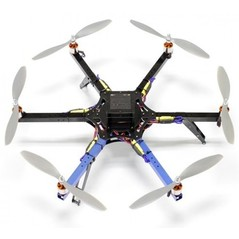
\includegraphics[width = 8cm]{fig/hexaCopter.jpg}
\caption{ArduCopter Hexacopter \textit{Courtesy arducopter.co.uk}}
\label{hexaCopter}
\end{figure}
\section{APM}
The APM is an open source flight control unit supporting multicopters, traditional helicopters, fixed wing aircraft and rovers \citep{devArdupilot}. Software is developed and supported by the DIYDrones community. At the moment the community has more than 45 000 members (November 2013) and an active forum where one could get help and useful tips and tricks.\\
\subsection{Modes of Operation}
The APM can operate in many different modes of operation \citep{flight}. The most relevant for this project are:
\begin{itemize}
\item Stabilize - Manual flight mode that automaticly levels the  UAV and maintains the current heading
\item Auto - The UAV tracks predefined waypoints
\item Guided - The next waypoint is defined in flight
\item RTL (Return to Launch) - The UAV returns to the position where it was armed and hovers
\item LAND - The UAV lands, shut-down the motors and disarms
\end{itemize}
Control signals in the different modes are given either with PWM-signals\footnote{Pulse Width Modulated signals} or through serial communication using the MAVLink protocol (the MAVLink protocol will be briefly explained below). The PWM-signals are usually sent from a 2.4 GHz radio via a receiver on the UAV, while the serial communication is usually sent from a ground station via a telemetry link to the APM. These signals could easily be replicated by the PandaBoard. A picture of the APM with a voltage regulator ann an external magnetometer and GPS module is found in Figure \ref{apm}.
\begin{figure}[H]
\centering
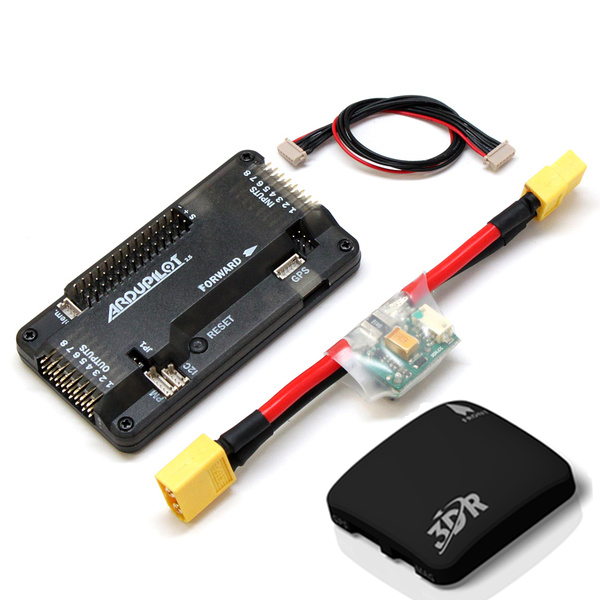
\includegraphics[width = 6cm]{fig/apm25.jpg}
\caption{APM 2.6 with a voltage regulator and an external magnetometer and GPS module \textit{Courtesy diydrones.com}}
\label{apm}
\end{figure}
\subsection{Sensors}
The APM is equipped with several sensors that are utilized for navigation and control. These will be briefly explained below.
\subsubsection{Barometer}
A barometer is an instrument that is used to measure air pressure \citep{barometer}. The barometric formula 
\begin{eqnarray}
p(h) = p(0)e^{-\dfrac{mgh}{kT}}
\label{barometer}
\end{eqnarray}
relates the pressure $p(h)$ of an isothermal, ideal gas of molecular mass $m$ at some height $h$ to its pressure $p(0)$ at height $h = 0$, where $g$ is the acceleration of gravity, $k$ the Boltzmann constant, and $T$ the temperature. This formula applies reasonably well to the lower troposphere. For altitudes up to 6 km the error is less than 5 \% \citep{Berberan-Santos1997}.\\
\newline
The barometer in the APM is based on piezoresistive technology. Piezoresisivity is a common sensing principle for micro machined sensor \citep{mems} that uses the fact that resistivity of some materials changes with applied stress \citep{Mason1957}. This feature is used in the barometer, when the air pressure varies, the pressure on the material in the barometer varies which means that resistivity varies. A mapping from resistivity to pressure is used to calculate altitude referenced to start altitude. Altitude calculations by the use of barometers can be sensitive to changing weather conditions.\\\newline
The barometer in the APM is the MS5611-01BA03 by Measurement Specialties, which according to the producer has a resolution of 10 cm.
\subsubsection{Magnetometer}
 A magnetometer is an instrument for measurement of magnetic fields. Depending on the setup they can measure strength of a magnetic field or both strength and direction of the field \citep{mag}. The magnetometer in the APM is a three-axes magnetometer. This means that both the strength and direction of the magnetic field can be measured. The magnetometer measures the force created by the magnetic field on an energized conductor. This force is called the Lorentz Force and follows the formula
 \begin{eqnarray}
 \boldsymbol{F} = q\boldsymbol{v} \times \boldsymbol{B}
 \label{bar}
 \end{eqnarray}
 where $q$ is charge, $\boldsymbol{F}$ is the Lorentz Force and $\boldsymbol{B}$ is the magnetic field. The charge $q$ is assumed to be known and $\boldsymbol{F}$ can be measured using piezoresistive principles. Then the magnetic field is easily found using the formula in equation (\ref{bar}). This field is pointing towards north (excluding disturbances from for instance the motors on the UAV), which will be utilized in the APMs IMU (described in the next section) to get more accurate attitude measurements.\\
\newline
The magnetometer in the APM is a HMC5883L from Honeywell.
\subsubsection{Inertial Measurement Unit}
The APM contains an Inertial Measurement Unit (IMU). An IMU consists of an ISA (Inertial Sensor Assembly), hardware and low level software. The ISA is a cluster of three gyroscopes and three accelerometers that measure angular velocity and acceleration respectively \citep{vik}. The IMU can also use magnetometer measurements. In the APM the magnetometer is not a part of the IMU, but it has an interface where it communicates with the magnetometer to make it possible to utilize the magnetometer measurements in the calculations of the attitude of the UAV.\\
\newline
Conceptually the accelerometer measures the movement of a damped mass hanging in a spring. To transform this movement into an electric signal, piezoresistive principles are utilized. In this case is it the acceleration that creates deformation in the piezoresistive material.\\
\newline
The gyroscopes are also based on MEMS technology. MEMS-gyroscopes are usually implemented with a tuning fork configuration. Two masses oscillate in opposite directions of each other. When these masses experiences angular velocity the Coriolis force act in opposite directions on the masses. This results in a measurable capacitance change which is proportional to the angular velocity of the UAV \citep{gyro}.\\
\newline
The IMU in the APM is a MPU-6000 from Inven Sense.
\subsubsection{GPS}
The GPS module that is connected to the APM contains an ublox LEA-6H module \citep{storeGPS}. It uses Navstar GPS but can also support GLONASS and Galileo. Communication to the APM is done via UART\footnote{Universal Asynchronous Receiver/Transmitter} with an update frequency of 5 Hz. Position accuracy is given by the datasheet to be 2.5 m CEP\footnote{CEP (Circular Error Probability) defines the radius of a circle centered in the true position containing 50 \% of the GPS measurements \citep{cep}}\citep{ublox}. GPS can also be used for altitude measurements, but the nature of the GPS is that altitude measurements will have even less accuracy than position measurements.
\subsection{Interfaces}
The APM has several interfaces that make it flexible and suitable for research and development. It has dedicated connection points for GPS and telemetry. These are interfaced using UART. It also has an unused UART-port available for other units and applications. Input from the radio and output for the motor controllers have dedicated ports that operates with PWM-signals. A connection point to access the APMs $I^2C$ bus is also available. Several units can communicate using this bus. It has also a lot of unused I/O-pins available for further development. These can for instance be used to connect an Ultrasonic Range Finder (there are several of them that are supported by the APM).
\subsubsection{MAVLink}
The APM communicates with its surroundings using UART with a subset of the communication protocol MAVLink\footnote{Micro Air Vehicle Communication Protocol}. MAVLink is a lightweight, header-only marshalling library for micro air vehicles \citep{mavlink}. MAVLink has a lot of predefined messages in addition to the possibility of creating custom messages. An XML-file contains the definition of the different message types. An example of one of the message definitions is shown in Figure \ref{mavlink}.
\begin{figure}[H]
\centering
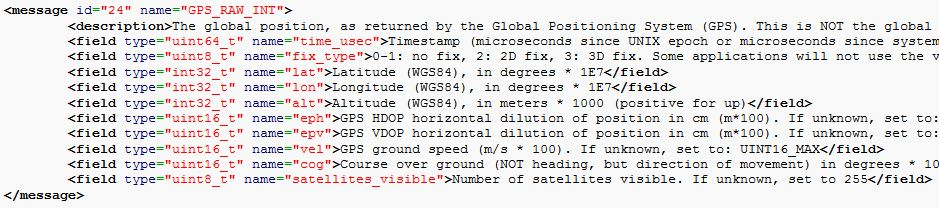
\includegraphics[width = 16cm]{fig/mavlink.JPG}
\caption{Message definition of message with ID 24 \textit{Courtesy of wikipedia.org}}
\label{mavlink}
\end{figure}\noindent
The MAVLink protocol can be used both to get status information from the APM and to give commands to the APM.
\section{PandaBoard ES}
The version of the PandaBoard used in this project is the PandaBoard ES Revision B2 (hereinafter referred to as PandaBoard). The PandaBoard is a small but powerful computer based on an OMAP$^{\rm TM}$ 4 Processor. The OMAP$^{\rm TM}$ 4 Processor is designed for high performance applications within a low power envelope \citep{omap} and contains a Dual-core ARM\textregistered  1.2 GHz CPU. The PandaBoard do also have 1 GB RAM and a port to insert a SD-card for additional memory \citep{panda}.
\subsection{Interfaces}
The PandaBoard has several interfaces that make it a good platform for development. It has two expansion connectors with 28 pins each. The functions of these pins includes general purpose I/O, SPI, $I^2C$, USB, UART, audio, power and support for additional memory \citep{pandaManual}. This means that the the PandaBoard is able of communicating with its surroundings using most of the most popular bus standards.\\
\newline
The PandaBoard does also include a camera header available for development of camera solutions. e-con Systems has developed a camera (e-CAM51\textunderscore 44x) especially for the PandaBoard and this header. The camera is a 5 MP auto focus camera able to provide 720p HD video streaming at 60 fps \citep{camera}. Communication with the camera uses the MIPI\footnote{Mobile Industry Processor Interface} CSI-2 standard. CSI-2 is a standard that provides a robust, scalable, low power and high speed interface for imaging solutions \citep{img}.  
%\begin{figure}[H]
%\centering
%\includegraphics[width = 8cm]{fig/cameraBoard.JPG}
%\caption{e-CAM51\textunderscore 44x(SOURCE: manual)}
%\end{figure}
\chapter{"Some chapter"}

\chapter{Background Theory}
\chapter{"Some implementation"}
\chapter{Testing and Results}
\section{Node Tracking}
\subsection{Result of Test}
\chapter{Discussion}
\chapter{Conclusion}
% Include more chapters as required.
%%=========================================
%\appendix
	% Include more appendices as required.
%%=========================================
\bibliographystyle{apa}
\addcontentsline{toc}{chapter}{\bibname}
\bibliography{bibtex/scopus}  
\end{document}